\chapter{Einige wichtige Hinweise zum Arbeiten mit \LaTeX\ }
\label{sec:latexumg}

Throughout this work the following notation is employed: $W$ denotes
the world frame, $C_1$ or $C_2$ denotes a camera frame.  $T_{AB}$ is
the transformation from frame $A$ to frame $B$, measured in frame $A$.

$\vec{X}$ the position of the event with respect to world or camera
frame, $\vec{x}$ the calibrated coordinates of the event.

\section{From Events to Frame}
\label{sec:event_warp}
We group a set of events $\mathscr{E}\doteq \{e_k\}_{k=1}^N$ into a
temporal window, optimize the motion and scene parameters within this
window, then shift the window to the next set of events and repeat
this process. The temporal window size is defined by the event numbers
$N$, which should be chosen small enough so that a constant velocity
model could be applied within this window. We choose event numbers
against a fixed time interval to define the window size, because this
corresponds to the data-driven nature of an event-based camera: the
more rapid the apparent motion of the scene is, the larger the event
rate will be. If the scene stops moving, no events will be generated,
the pose will also not be further updated.

An event frame is thus formed by summing up events within this
window. If we simply sum along the time axis, the intensity at each
pixel will be the sum of the polarities of all the events that are
triggered at this pixel location within the window
\begin{equation}
  \label{eq:intensity}
  \mathcal{I}(\vec{x}) = \sum_1^N\pm_k(\vec{x}-\vec{x}_k),
\end{equation}
with $\pm_k$ and $\vec{x}_k$ denoting the polarity and pixel
coordinates of the $k$th event, respectively. After warping the events
with $\vec{x}'_k=\mat{W}(\vec{x}_k,t;\theta)$, we substitute
$\vec{x}_k$ in the above equation to $\vec{x}'_k$.
\subsection{Planar Homography}

\label{sec:planar_homo}
The warp function $\vec{x}'=\mat{W}(\vec{x},t;\theta)$ does
not only depend on the motion parameters, but also the scene
parameters, which is the unknown depth.  In the case of a planar scene
the problems simplifies, since a plane $\mathbf{P}$ can be
parameterized by two sets of parameters: $\vec{n}\in\mathbb{S}^2$ the
unit surface normal of $\mathbf{P}$ with respect to the current camera
frame, and $d$ the distance from the camera center to
$\mathbf{P}$. The warp function then becomes
\begin{align}
  \label{eq:planar_homo}
  \vec{X}=&\mat{R}\vec{X}'+\vec{T}\\
  \vec{X}'=&\mat{R}^\top\left(\vec{X}-\vec{T}\right)\\
  \vec{X}'=&\mat{R}^\top\left(\mat{I}+\vec{T}\vec{n}^\top/d\right)\vec{X},
\end{align}
thus
$\vec{x}'\sim\mat{R}^\top\left(\mat{I}+\vec{T}\vec{n}^\top/d\right)\vec{x}$.
Here $(\mat{R}, \vec{T})\in SE(3)$ denotes the relative pose between
two cameras at which the current event being warped and the first
event within the window happened. Under a constant velocity model with
linear velocity $\vec{v}\in\mathbb{R}^3$ and angular velocity
$\bm{\omega}\in\mathbb{R}^3$, the translation is given by
\begin{equation}
  \label{eq:translation}
  \vec{T}(t)=\vec{v}t,
\end{equation}
the rotation matrix is given by the \textit{exponential map} exp:
$\mathfrak{so}(3)\rightarrow SO(3)$:
\begin{equation}
  \label{eq:rotation}
  \mat{R}(t)=\mathrm{exp}(\bm{\omega}^\wedge t),
\end{equation}
where $^\wedge$ is the \textit{hat} operator
\begin{equation}
  \label{eq:hat}
  \bm{\omega}^\wedge=
  \begin{bmatrix}
    \omega_1\\\omega_2\\\omega_3
  \end{bmatrix}
  =
  \begin{bmatrix}
    0&-\omega_3&\omega_2\\
    \omega_3&0&-\omega_1\\
    -\omega_2&\omega_1&0
  \end{bmatrix}
  \in\mathfrak{so}(3),
\end{equation}

\section{From Frames to Map}
\label{sec:mapping}
The procedure in the above section optimizes the relative pose between
successive frames.


\section{Gliederungen}
\label{sec:gliederung}

Ein Text kann mit den Befehlen \texttt{\textbackslash chapter\{.\}},
\texttt{\textbackslash section\{.\}}, \texttt{\textbackslash
  subsection\{.\}} und \texttt{\textbackslash subsubsection\{.\}}
gegliedert werden.


\section{Referenzen und Verweise}
\label{sec:refverw}

Literaturreferenzen werden mit dem Befehl \texttt{\textbackslash
  citep\{.\}} und \texttt{\textbackslash citet\{.\}}
erzeugt. Beispiele: ein Buch
\citep{Raibert1986LeggedRobotsThatBalance}, ein Buch und ein Journal
Paper
\citep{Raibert1986LeggedRobotsThatBalance,Vukobratovic2004ZeroMomentPoint},
ein Konferenz Paper mit Erwähnung des Autors: \citet{Pratt1995SEA}.

Zur Erzeugung von Fussnoten wird der Befehl \texttt{\textbackslash
  footnote\{.\}} verwendet. Auch hier ein Beispiel\footnote{Bla bla.}.

Querverweise im Text werden mit \texttt{\textbackslash label\{.\}}
verankert und mit \texttt{\textbackslash cref\{.\}} erzeugt.  Beispiel
einer Referenz auf das zweite Kapitel: \cref{sec:latexumg}.


\section{Aufzählungen}\label{sec:aufz}

Folgendes Beispiel einer Aufzählung ohne Numerierung,
\begin{itemize}
\item Punkt 1
\item Punkt 2
\end{itemize}
wurde erzeugt mit:
\begin{verbatim}
\begin{itemize}
\item Punkt 1
\item Punkt 2
\end{itemize}
\end{verbatim}

Folgendes Beispiel einer Aufzählung mit Numerierung,
\begin{enumerate}
\item Punkt 1
\item Punkt 2
\end{enumerate}
wurde erzeugt mit:
\begin{verbatim}
\begin{enumerate}
\item Punkt 1
\item Punkt 2
\end{enumerate}
\end{verbatim}

Folgendes Beispiel einer Auflistung,
\begin{description}
\item[P1] Punkt 1
\item[P2] Punkt 2
\end{description}
wurde erzeugt mit:
\begin{verbatim}
\begin{description}
\item[P1] Punkt 1
\item[P2] Punkt 2
\end{description}
\end{verbatim}


\section{Erstellen einer Tabelle}\label{sec:tabellen}

Ein Beispiel einer Tabelle:
\begin{table}[h]
  \begin{center}
    \caption{Daten der Fahrzyklen ECE, EUDC, NEFZ.}\vspace{1ex}
    \label{tab:tabnefz}
    \begin{tabular}{ll|ccc}
      \hline
      Kennzahl & Einheit & ECE & EUDC & NEFZ \\ \hline \hline
      Dauer & s & 780 & 400 & 1180 \\
      Distanz & km & 4.052 & 6.955 & 11.007 \\
      Durchschnittsgeschwindigkeit & km/h & 18.7 &  62.6 & 33.6 \\
      Leerlaufanteil & \% & 36 & 10 & 27 \\
      \hline
    \end{tabular}
  \end{center}
\end{table}

Die Tabelle wurde erzeugt mit:
\begin{verbatim}
\begin{table}[h]
  \begin{center}
    \caption{Daten der Fahrzyklen ECE, EUDC, NEFZ.}\vspace{1ex}
    \label{tab:tabnefz}
    \begin{tabular}{ll|ccc}
      \hline
      Kennzahl & Einheit & ECE & EUDC & NEFZ \\ \hline \hline
      Dauer & s & 780 & 400 & 1180 \\
      Distanz & km & 4.052 & 6.955 & 11.007 \\
      Durchschnittsgeschwindigkeit & km/h & 18.7 &  62.6 & 33.6 \\
      Leerlaufanteil & \% & 36 & 10 & 27 \\
      \hline
    \end{tabular}
  \end{center}
\end{table}
\end{verbatim}


\section{Einbinden einer Grafik}\label{sec:epsgraph}

Das Einbinden von Graphiken kann wie folgt bewerkstelligt werden:
\begin{verbatim}
\begin{figure}
  \centering 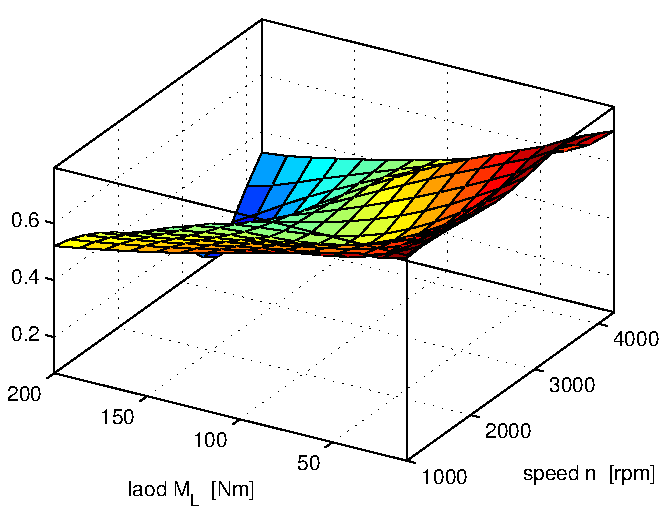
\includegraphics[width=0.75\textwidth]{images/k_surf.pdf}
  \caption{Ein Bild.}
  \label{fig:k_surf}
\end{figure}
\end{verbatim}

\begin{figure}
  \centering 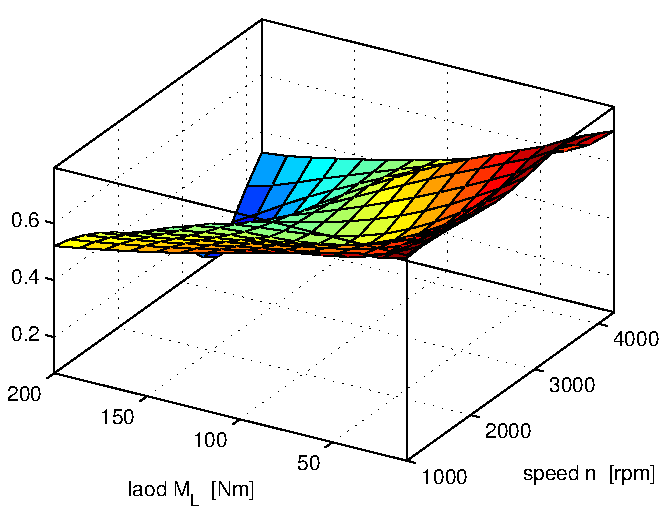
\includegraphics[width=0.75\textwidth]{images/k_surf.pdf}
  \caption{Ein Bild}
  \label{pics:k_surf}
\end{figure}

oder bei zwei Bildern nebeneinander mit:
\begin{verbatim}
\begin{figure}
  \begin{minipage}[t]{0.48\textwidth}
    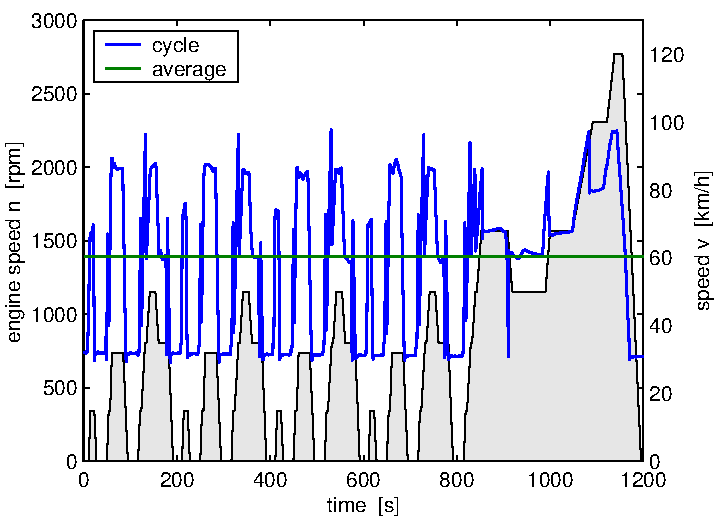
\includegraphics[width = \textwidth]{images/cycle_we.pdf}
  \end{minipage}
  \hfill
  \begin{minipage}[t]{0.48\textwidth}
    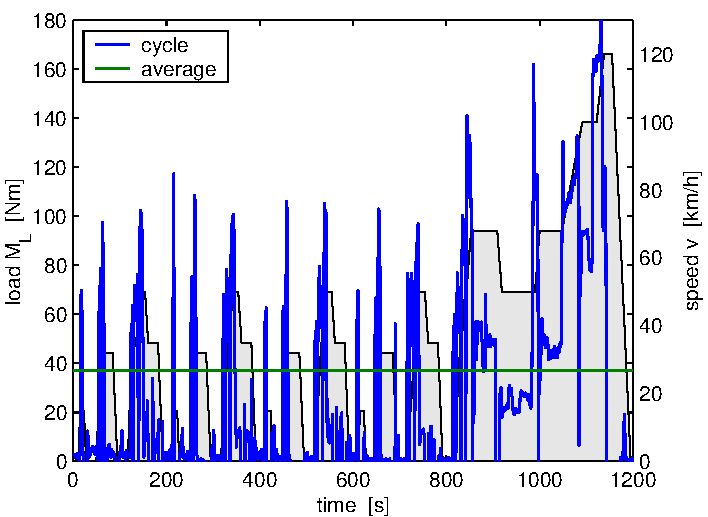
\includegraphics[width = \textwidth]{images/cycle_ml.pdf}
  \end{minipage}
  \caption{Zwei Bilder nebeneinander.}
  \label{pics:cycle}
\end{figure}
\end{verbatim}

\begin{figure}
  \begin{minipage}[t]{0.48\textwidth}
    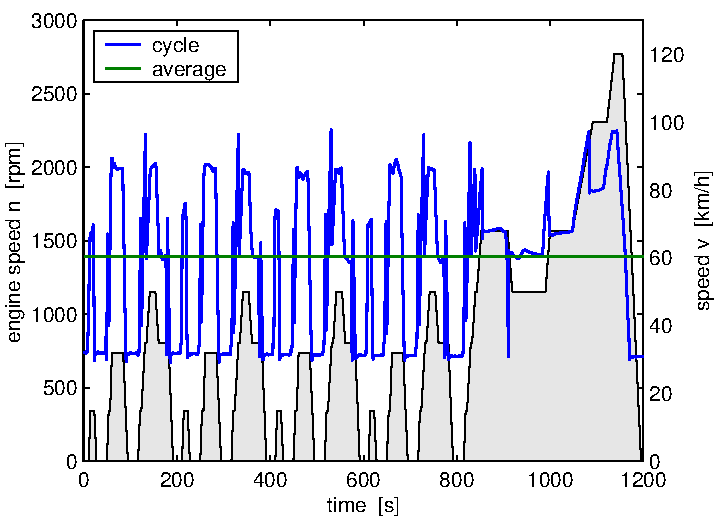
\includegraphics[width = \textwidth]{images/cycle_we.pdf}
  \end{minipage}
  \hfill
  \begin{minipage}[t]{0.48\textwidth}
    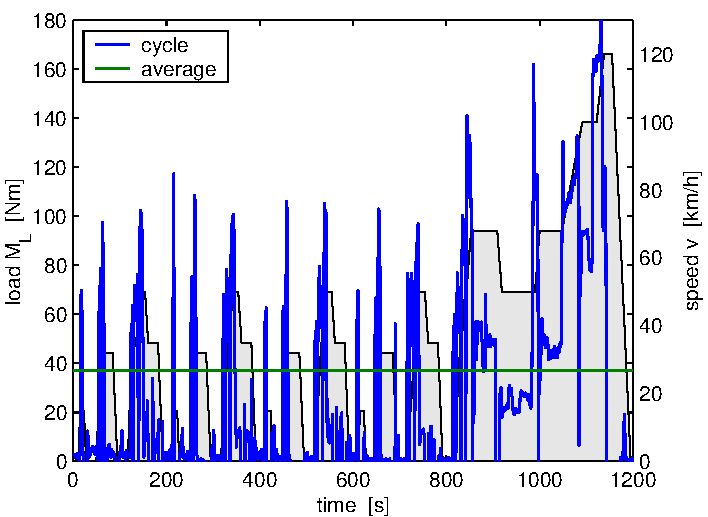
\includegraphics[width = \textwidth]{images/cycle_ml.pdf}
  \end{minipage}
  \caption{Zwei Bilder nebeneinander}
  \label{pics:cycle}
\end{figure}


\section{Mathematische Formeln}\label{sec:math}

Einfache mathematische Formeln werden mit der equation-Umgebung
erzeugt:
\begin{equation}
  p_{me0f}(T_e,\omega_e) \ = \ k_1(T_e) \cdot (k_2+k_3 S^2
  \omega_e^2) \cdot \Pi_{\mathrm{max}} \cdot \sqrt{\frac{k_4}{B}} \, .
  \label{eq:my_equation}
\end{equation}

Der Code dazu lautet:
\begin{verbatim}
\begin{equation}
  p_{me0f}(T_e,\omega_e) \ = \ k_1(T_e) \cdot (k_2+k_3 S^2
  \omega_e^2) \cdot \Pi_{max} \cdot \sqrt{\frac{k_4}{B}} \, .
\end{equation}
\end{verbatim}

Mathematische Ausdrücke im Text werden mit \$formel\$ erzeugt (z.B.:
$a^2+b^2=c^2$).

Vektoren und Matrizen werden mit den Befehlen \texttt{\textbackslash
  vec\{.\}} und \texttt{\textbackslash mat\{.\}} erzeugt
(z.B. $\vec{v}$, $\mat{M}$).


\section{Weitere nützliche Befehle}\label{sec:div}

Hervorhebungen im Text sehen so aus: \emph{hervorgehoben}. Erzeugt
werden sie mit dem \texttt{\textbackslash epmh\{.\}} Befehl.

Einheiten werden mit den Befehlen \texttt{\textbackslash unit[1]\{m\}}
(z.B.~\unit[1]{m}) und \texttt{\textbackslash unitfrac[1]\{m\}\{s\}}
(z.B.~\unitfrac[1]{m}{s}) gesetzt.
